Il est possible de naviguer dans le menu à partir de tous les contrôleurs ayant été détectés.
Voici les touches et boutons défini pour naviguer dans les différents menus de l'application : \\

	Pour le clavier, les touches directionnelles permettent de se déplacer dans le menu, les touches entrée et echap permettent respectivement de valider et d'annuler.
	
	
	Pour les autres contrôleurs, voici la configuration prédéfinie :

\begin{figure}[h]
	\begin{center}
		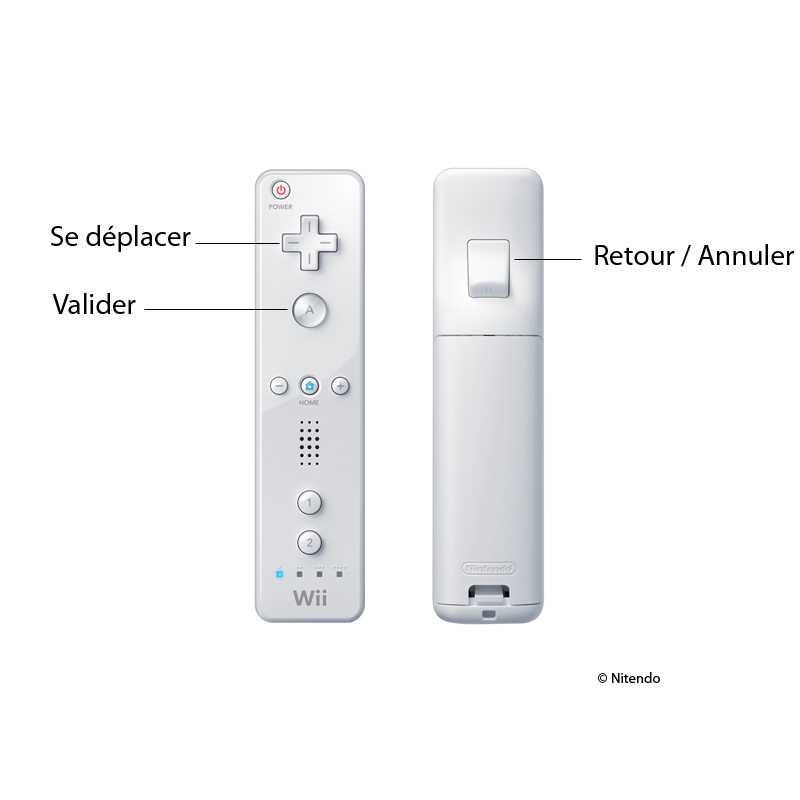
\includegraphics[scale=0.9]{images/wii_menu.png}
		\caption{Naviguer dans le menu avec une wiimote}
	\end{center}
\end{figure}

\begin{figure}[h]
	\begin{center}
		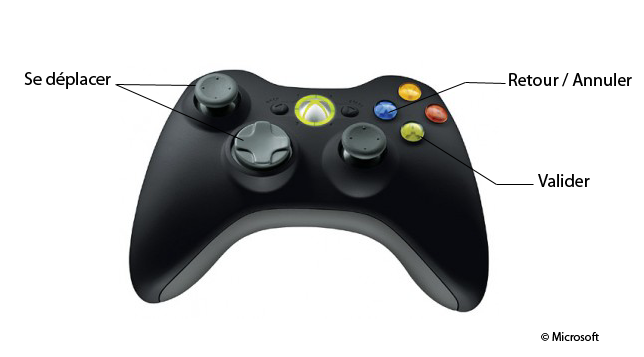
\includegraphics[scale=0.3]{images/gamepad_menu.png}
		\caption{Naviguer dans le menu avec un joystick}
	\end{center}
\end{figure}

